%%%%%%%%%%%%%%%%%%%%%%%%%%%%%%%%%%%%%%%%%
% Thin Sectioned Essay
% LaTeX Template
% Version 1.0 (3/8/13)
%
% This template has been downloaded from:
% http://www.LaTeXTemplates.com
%
% Original Author:
% Nicolas Diaz (nsdiaz@uc.cl) with extensive modifications by:
% Vel (vel@latextemplates.com)
%
% License:
% CC BY-NC-SA 3.0 (http://creativecommons.org/licenses/by-nc-sa/3.0/)
%
%%%%%%%%%%%%%%%%%%%%%%%%%%%%%%%%%%%%%%%%%

%----------------------------------------------------------------------------------------
%	PACKAGES AND OTHER DOCUMENT CONFIGURATIONS
%----------------------------------------------------------------------------------------

\documentclass[a4paper, 11pt]{article} % Font size (can be 10pt, 11pt or 12pt) and paper size (remove a4paper for US letter paper)

\usepackage[protrusion=true,expansion=true]{microtype} % Better typography
\usepackage{graphicx} % Required for including pictures
\usepackage{wrapfig} % Allows in-line images
\usepackage{gensymb}
\usepackage{caption}
\usepackage{subcaption}
\usepackage{rotating}

\usepackage{mathpazo} % Use the Palatino font
\usepackage[T1]{fontenc} % Required for accented characters
\linespread{1.05} % Change line spacing here, Palatino benefits from a slight increase by default

\makeatletter
\renewcommand\@biblabel[1]{\textbf{#1.}} % Change the square brackets for each bibliography item from '[1]' to '1.'
\renewcommand{\@listI}{\itemsep=0pt} % Reduce the space between items in the itemize and enumerate environments and the bibliography

\renewcommand{\maketitle}{ % Customize the title - do not edit title and author name here, see the TITLE block below
\begin{flushright} % Right align
{\LARGE\@title} % Increase the font size of the title

\vspace{50pt} % Some vertical space between the title and author name

{\large\@author} % Author name
\\\@date % Date

\vspace{40pt} % Some vertical space between the author block and abstract
\end{flushright}
}

%----------------------------------------------------------------------------------------
%	TITLE
%----------------------------------------------------------------------------------------

\title{\textbf{The Stallion}\\ % Title
Group 9 Project Report\\DD2425} % Subtitle

\author{\textsc{
Tobias Andersson\\
Max Losch\\
Diego Martinez Marrodan\\
Tiago Sebastiao\\
Lan Wang} % Author
\\{\textit{Royal Institute of Technology}}
} % Institution

\date{\today} % Date

%----------------------------------------------------------------------------------------

\begin{document}

\maketitle % Print the title section

%----------------------------------------------------------------------------------------
%	ABSTRACT
%----------------------------------------------------------------------------------------

%\renewcommand{\abstractname}{Summary} % Uncomment to change the name of the abstract to something else

\begin{abstract}

This report describes the design decisions, accomplishments and evaluation of the work done by Group 9 during the course DD2425 Robotics and Autonomous Systems. 
In summary the robot uses an occupancy grid and a topoloical map to navigate in the maze, and the 3D information from the primesense camera together with PCL for object recognition.
In the end the system worked well enough to solve the whole task in simple cases.

\end{abstract}

\newpage
\tableofcontents
\newpage

%----------------------------------------------------------------------------------------
%	ESSAY BODY
%----------------------------------------------------------------------------------------

\section{About The Robot}
\subsection{Robot Structure}

The construction of our robot, which is called The Stallion(or Cute Girl), took about 1.5 weeks.
We managed to make the robot structure as compact as possible, so that it can get more freedom within the maze.
The dimention of the robot can be seen as below.

%\begin{figure} 
%  \centering 
%  \subfigure[A]{ 
%    \label{fig:subfig:a} %% label for first subfigure 
%    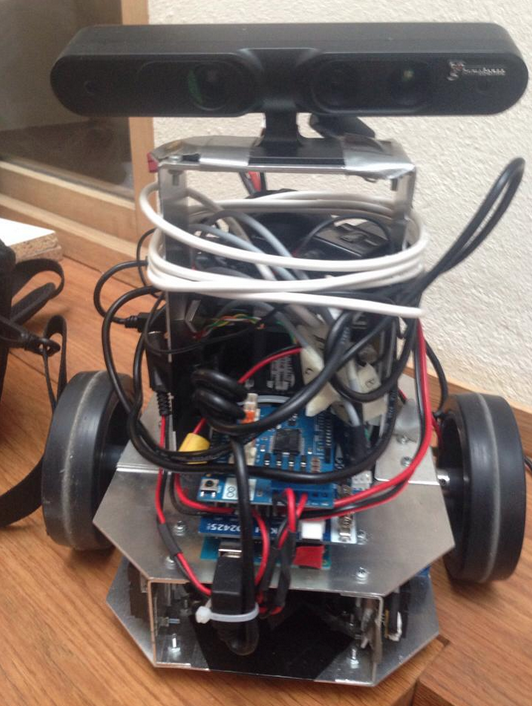
\includegraphics[width=1.0in]{robot.jpg}} 
%  \hspace{1in} 
%  \subfigure[Big Box]{ 
%    \label{fig:subfig:b} %% label for second subfigure 
%    \includegraphics[width=1.5in]{dimentions.png}} 
%  \caption{Two Subfigures} 
%  \label{fig:subfig} %% label for entire figure 
%\end{figure}
\begin{figure}[h]
\centering
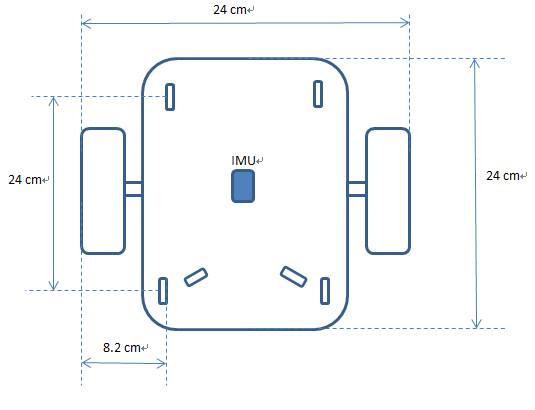
\includegraphics[width=8cm]{figures/dimensions.jpg}
\caption{Robot Top View and Sensor Plancement} 
\end{figure}

\setlength{\parindent}{0pt}Since the robot is constructed with the same length and width of 24cm, when it turns, it will never hit the front wall as long as there was space left in front before it turns.
The robot has two layers. On the bottom layer, motors, wheels are mounted in the center and all sensors are fixed on this layer as well.
On the top layer,the Arduino board, the camera braket are fixed.
Also there are two big holes on the top layer, where fits perfectly in the NUC and the battery.
While since the NUC is actually standing between two layers with its USB connectors facing sideways, the connectors almost touched the wheels.
This problem was fixed by hanging the cables tightly upwards.
It was good that we didn't rebuild the robot or spend lots of time on modification of the mechanical structure with the project proceeding. 

\subsection{Sensor Placement}
There are 6 IR sensors, one IMU sensor integrated on the robot.
On each side of the robot,two short range IR sensors are mounted with distance inbetween as far as possible, in order to get a better esitmation of the robot angle. 
And two long range IR sensors pointed to the front with an angle adjustment to the robot center.  
The reason why the front IR sensors are not pointed directly to the front is because if we do that, when there are obstacles come to the area exactly between the two front sensors, nothing will be detected.
With crossed sensors,an triangle area will be formed,thus it guarantees front obstacle detection.
Actually, we took advantages of such placement when dealing with the 'wall of death '.\\

\setlength{\parindent}{0pt}There is also an IMU sensor mounted on the bottom layer, we used it for detection of crash.When the robot crashes into an obstacle, the IMU will send the current time to brain to reset.
And the robot will try to go backwards and continue it's path again.

\subsection{Camera Placement}
Since the PrimeSense has a minimal working range of 35 cm, the camera is fixed on top of an aluminium tower with height of 28cm above the floor. 
The system is not sensitive to the camera angle since software calibration of camera angle will be executed when the vision is started.
Thus we are able to give position of detected objects precisely without caring a lot about the camera angle.
\section{Controlling}

The main task of the project requires the robot to move with the highest possible speed.
On the other hand the robot should be able to move at a speed that induces as little drift as possible and reduces the risk of errors when hitting an obstacle.
And lastly, the vision would have to identify objects from further away, increasing the difficulty of implementation and recognition.
Thus, a balance in the velocities have to be found.\\

The implemented controllers consisted of a forward movement controller, a turn controller and a wall alignment controller.
By embedding them in an adapter pattern it was possible to render their usage very versatile (see figure \ref{fig:arch_controller}).
Every controller inherited hereby a controller base which defined an interface that updated the logic and returned a Twist
(A Twist is one of many ros pre-baked data structures that can be sent as a message. 
It stores a position and a rotation). 
The adapter combines all received Twists to one Twist, entrusting that no contradictions occur.
A top logic has to ensure that the right controllers are activated and deactivated.
This can be done by activating and deactivating each controller.
Controllers like the turn and the forward movement controller respond with a message as soon as they have stopped or finished their activity.\\

\begin{figure}[h]
\begin{center}
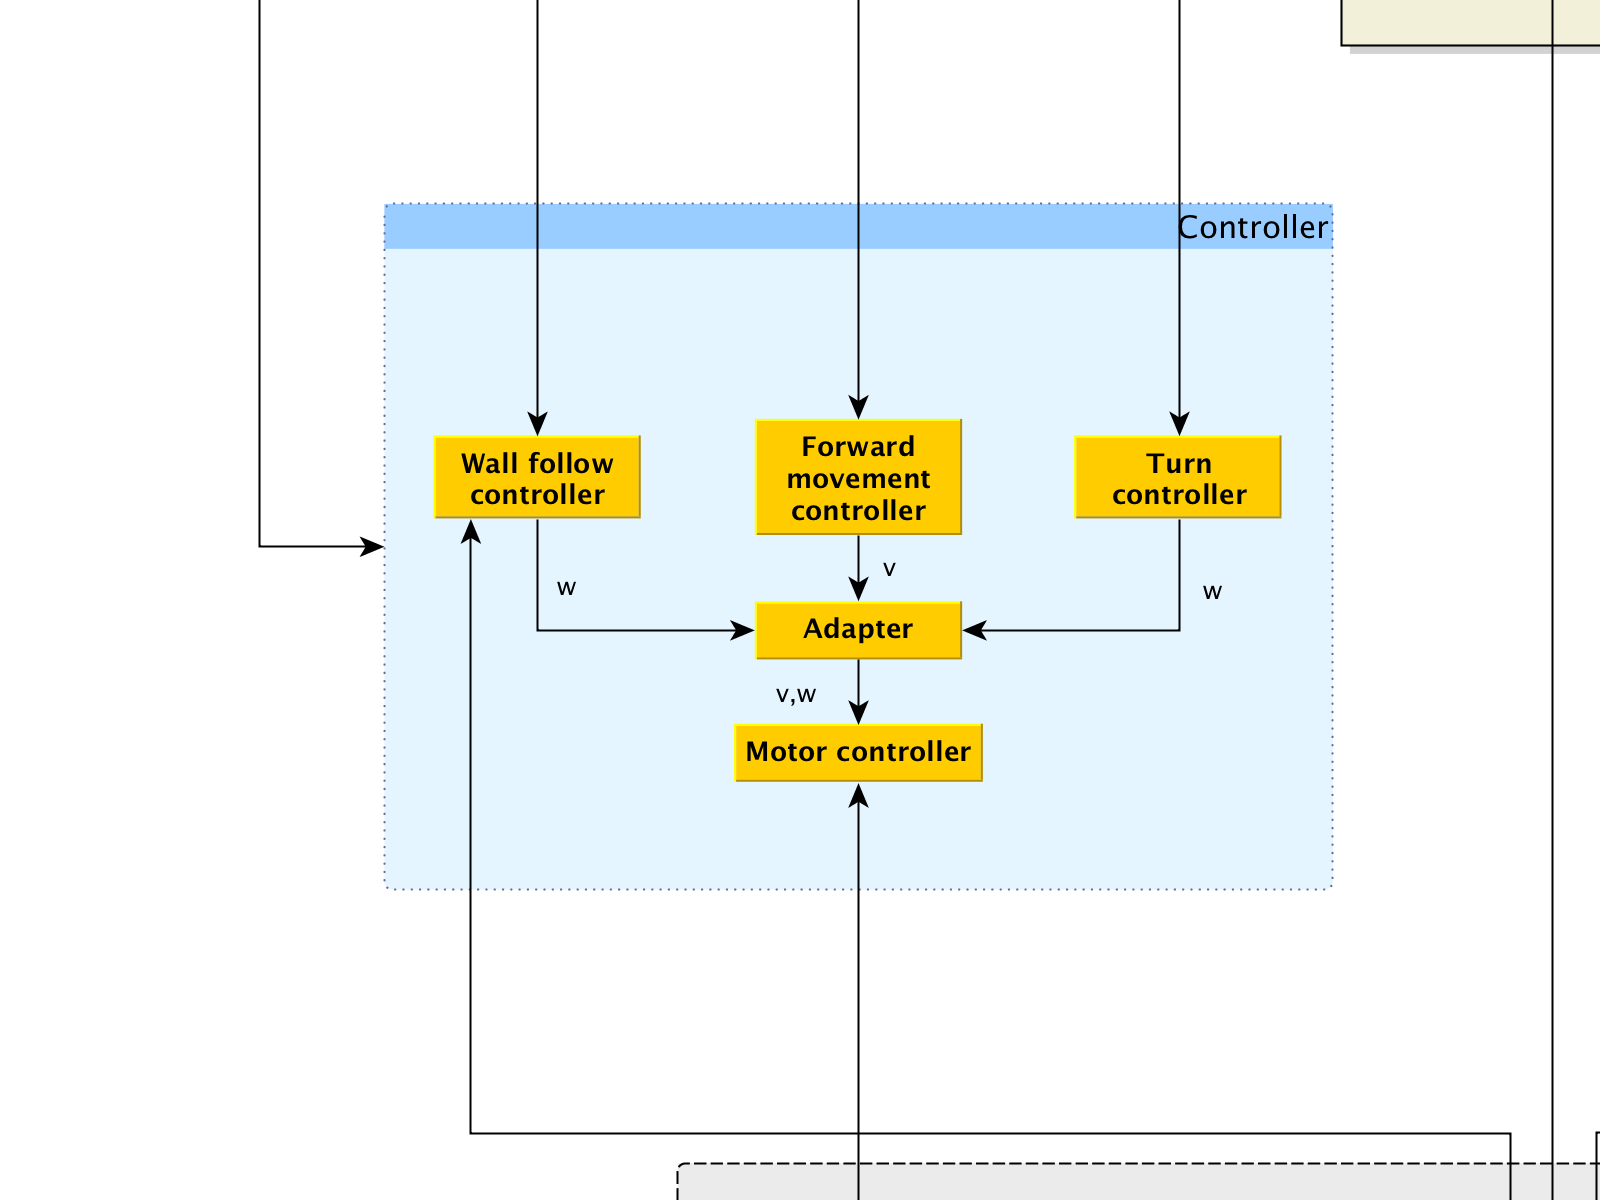
\includegraphics[width=0.6\textwidth]{figures/arch_controller.png}
\end{center}
\caption{Architecture of the controller package}
\label{fig:arch_controller}
\end{figure}

\subsection{Motor controller}

Due to internal motor difference, it is not sufficient to control the motors directly.
Otherwise the robot would move in an arch, one motor rotating slower than the other.
To compensate for that and to also be able to input linear and angular velocities, a PID controller was used. 
This enabled the robot to drive in a stable straight line.

The motors itself have a static resistance, that have to be overcome whenever the motors should transition from idling to rotating.
Overcoming these static resistance could be described by constants (for each motor one) $K_{power}$, that were added to the result of the PID results.
As soon as the static resistance has been overcome and the motor is rotating, the constant $K_{power}$ can be reduced to a value that sustains rotation: $K_{sustain}$.
This behavior results in a spiked motor control output as can be seen in figure \ref{fig:pwm_spiker}.
Although movement without spiking is possible due to the accumulating behavior of the PID controller too, it ensures responsive controlling and avoids the necessecity of increasing the gains which can easily result in overshoots.

\begin{figure}[h]
\begin{center}
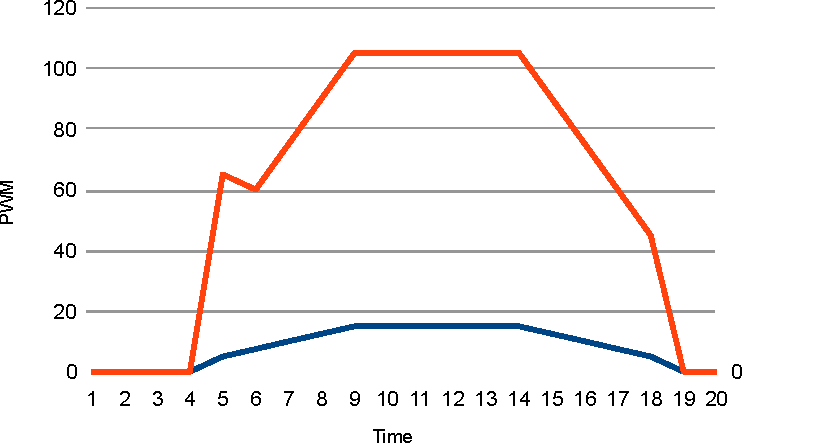
\includegraphics[width=0.6\textwidth]{figures/pwm_spike.pdf}
\end{center}
\caption{PWM Spiking for initial motor rotation attempt}
\label{fig:pwm_spiker}
\end{figure}

\subsection{Wall alignment}

The wall allignment controller (see figure \ref{fig:arch_controller}) uses the IR sensors to measure the distances from the robot to the walls, and works as follows: if both walls are close to the robot (distance < 0.4 m), then keep the robot aligned to the center between both walls.
Otherwise control only by the next closest wall, or if no wall is present, do not align.
\input{sections/Localization}
\input{sections/Mapping}
\section{Vision}

Although the main intent of the vision was to detect the given set of objects (see figure \ref{fig:object_set},
it was later on also used to exploit wall and ground information for mapping and localization functionality.

\begin{figure}
\begin{center}
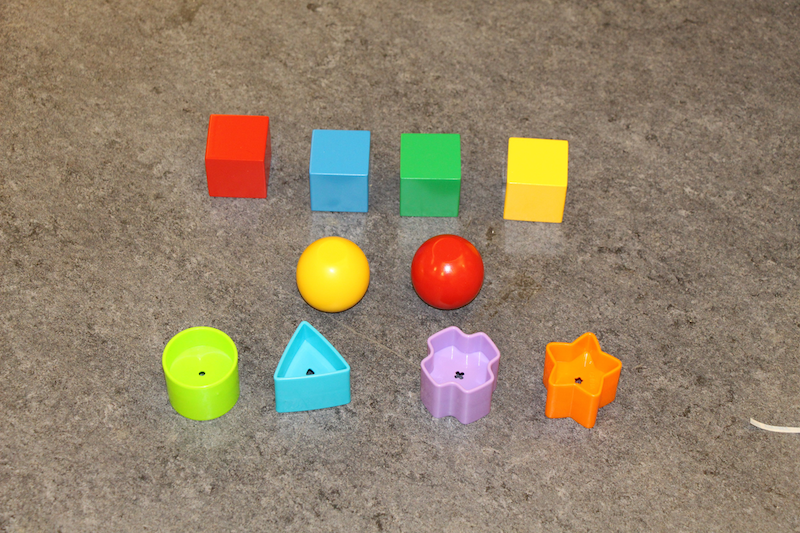
\includegraphics[width=0.38\textwidth]{figures/object_dataset}
\end{center}
\caption{Object data set}
\label{fig:object_set}
\end{figure}

The vision part of the project can be divided in 3 different parts.
They are object detection, shape recognition and color recognition.
While both shape and color recognition both rely on the accuracy and overall results of the object detection algorithm, they are totally independent. 
The final result of the whole object recognition part of the project is done after having reliable data form each of the components, color and shape.
In this part we chose to implement everything upon the Point Cloud Library. 
This choice is based on the added functionality of actually being able to represent the objects and walls and ground by points in 3D and not in a 2D picture. 
And such having more information about the object structure and additionally being less dependent on illumination changes.
Of course it is possible to convert between these two representations, but the PCL library has already a lot of useful functions that were able to decrease the amount of data manipulation.

\subsection{Object Detection}

The main idea is that we know that the objects are at ground level.
If we can detect the ground, we can then set some boundaries on the presence of the object above it, hence increasing the chances of detecting an object.
So the first part was find the walls and ground. Here, RANSAC was used. This algorithm exploits the fact that we are trying to find a special kind of order (model) among our data.
In our case, our data is the point cloud at a given time and the model are planes. 
By trying to fit planes in the point cloud, the algorithm is able to distinguish between inliers, points in some specific plane, and outliers, like noise or indeed the objects we are trying to find.
Now that we have the ground plane, we define a region of interest of about 5 cm high above it, where, if we can detect enough points, we will group them and afterwards classify them.
Note that it is possible to have 2 objects that satisfy the ground distance criteria and hence the conditions for an interesting group of points to exist is constrained by its size.
When this algorithm ends, we know one of two things:
\begin{enumerate}
\item there is no object in the frame
\item there is at least one region of interest
\end{enumerate}

\begin{figure}
\begin{center}
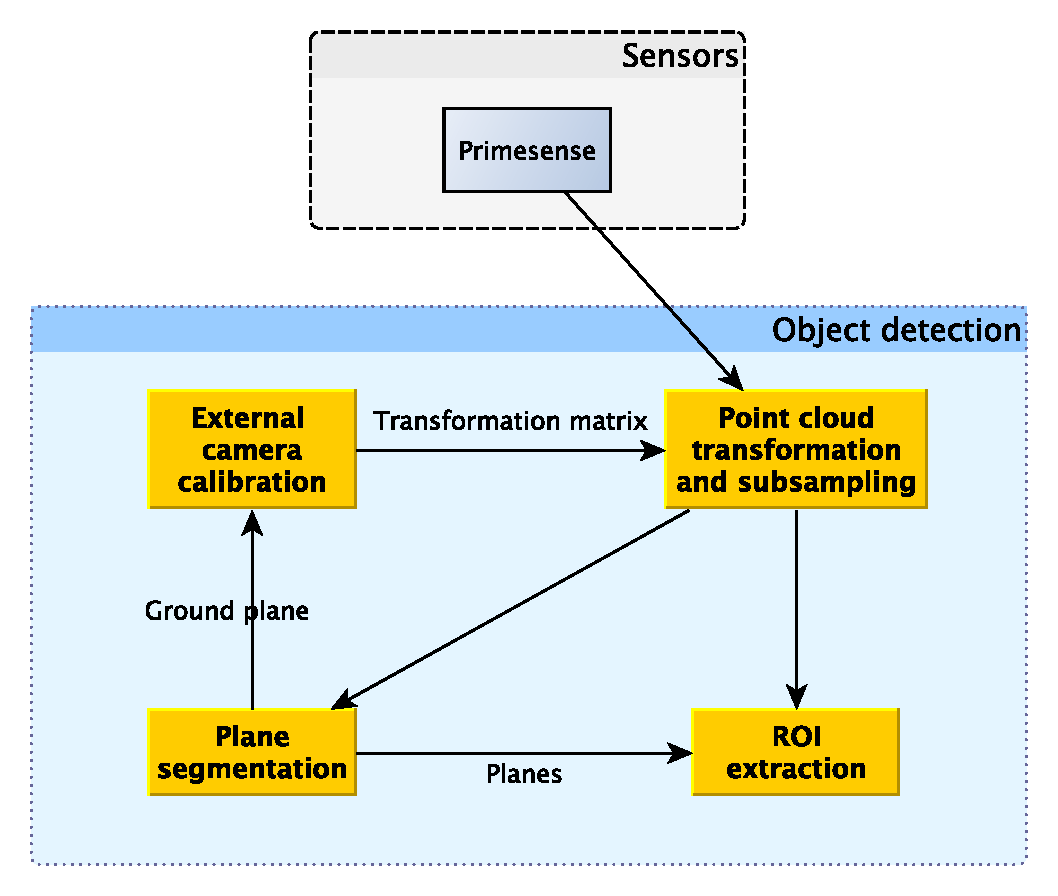
\includegraphics[width=0.45\textwidth]{figures/arch_vision_obj_det.pdf}
\end{center}
\caption{Object detection - Process flow}
\label{fig:vision:obj_det}
\end{figure}
 
\subsection{Object recognition} 
 
\subsection{Shape Recognition}

In this section we explain our logic behind the shape recognition algorithm.
The general idea was again model fitting.
We know about 3 very specific models that we want to try, cube, cylinder and sphere, and we have two objects with no general model.
The PCL library has available the RANSAC algorithm to fit some predifined models, like planes, spheres and cylinders. 
And that is what we used. 
The sphere fitting and cylinder are straightforward since they work exactely like the plane fitting mentioned above, the only difference being that the model is no longer a plane.
Hence they work in similar way as the plane fitting.
The big difference is the cube.
To recognize a cube we do plane fitting too, but we impose some conditions of the planes.

\begin{enumerate}
\item if 3 planes are detected then it's a cube
\item there has to be a parallel plane relative to the ground
\item distance between the ground plane and the parallel plane described above must be reasonable
\item the furthest plane must be the parallel plane
\end{enumerate}

The constraints above limit the possibility of noise being misclassified, as well as other shapes being mischaracterized.
There was obviously some empirical testing in order to find the best parameters for the RANSAC model fitting, like: 

\begin{itemize}
\item MAX:: I know some of them but can't remember their function
\end{itemize}


\subsection{Color Recognition}

Extracting the color values from an image, or in our case from points, is not a hard task. 
However, to give meaning to those values is harder, since the color itself depends on a rather large number of factors like available light, its intensity, its color, among others.
This makes it hard to obtain a robust but consistent color recognition algorithm.
Our approach was very empirical. The analysis is made per color possible and not all at once, even though the algorithm is the same whatever the color.
We started by analising the HSV (hue, saturation, value) values we got from the regions of interest, mainly the hue, which is what defines the color. 
We then tried to find meaning in those values, mainly their average.
We concluded that for the most part, the overall average of hues of all the points in the region of interest would be enough to obtain a good estimate of the color. 
So we defined an area our each color mean value around which the color will be.
The bigger the margin, the more robust the algorithm would be.
However, because of the specific colors, the margin could not be too large, or the added robustness would not be reliable, as colors would start to mix.
Because different conditions may lead to very different results, we weighted two times the previous result based on specific situations, mainly, the percentage of points that have the color being tested relative to the total number of points, and the probability of being of the color being analysed, i.e., considering the point clouds don't usually have that many points, we give a higher weight to probabilities above a certain value.
Because the blob of interest may have points not only belonging to the object we want, but also from the ground or wall (if the object is very close to one), the number of points that have a color similar to orange, color of the ground, is also relevant in deciding the true color of the object, and hence helps in determining the weight of the probability of the color being analysed.
The end result is a somewhat robust algorithm and consistent as far as our testing went. 

\begin{figure}
\begin{center}
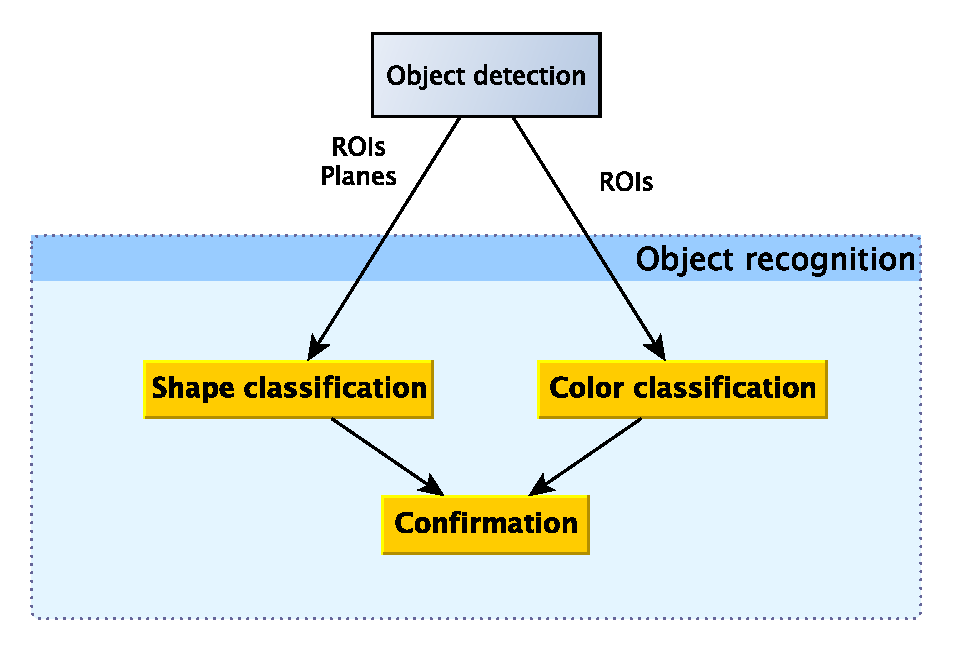
\includegraphics[width=0.45\textwidth]{figures/arch_vision_obj_rec.pdf}
\end{center}
\caption{Object recognition - Process flow}
\label{fig:vision:obj_rec}
\end{figure}
\section{Exploration}

The robot is controlled by a master node called the ``brain''. 
The brain is a state machine that is implemented with a the ROS package SMACH. 
In order to use SMACH the brain had to be implemented in python and it is the only node in the project which does not use C++.
The basic strategy of the brain is to go forward until it detects something interesting. 
When an obstacle is encountered, it turns left, right, or back in order of prefrence. 
When an object is detected the brain will go closer or further away from the object to reach the optimal recognition distance, then turn towards the object, and then activate the recognition, to attempt to recognize the object.
When a previously visited node is detected the brain will enter follow graph mode.
Follow graph mode will take the robot to the closest unexplored area in phase one, and will follow the whole TSP tour and visit all objects in phase two.
The brain also has a state to recover from a crash reported by the IMU, which is sadly a little too unsophisticated, but still helps quite a lot. When a crash is detected the state of the brain will be reset, i.e. stop, and reset all flags. Then the robot will back away from the crash site, turn towards the direction at the current node that is unexplored (if any), and then resume operation.


\section{Performance}
Our system did perform reasonably well in the end, and managed to get us third place in the competition. 
We have all the parts required to perform the main task of the project, i.e. navigate in the maze and recognize objects, return to the start, and then fetch the objects using the map constructed in the first phase. 
Sadly we did not have time to test the phase two logic in time for the competition, and it was therefore not used.
The whole system together only works well in simple mazes though. 
Since some parts of the system are not robust enough, the chance of everything working fully at the same time is not very high in the hard part of the maze. 

Control works alright, but could be better. 
We can't move as fast some other groups, because of the high risk of crashing. 

Mapping and navigation works very well, drift in the map is never a problem unless we crash. Sometimes we place too many nodes in open areas, which results in time being wasted on pointless exploration.

The vision worked well for the simple objects, but we can't recognize the hollow objects when standing still. 
Experiments were made with a ``shake controller'' that should shake the robot back and forth when detecting an object, but that did not work well enough.

Integration worked fine until the end when we added a lot of features that needed to be integrated really fast. Then it got messy very quickly and not robust enough.ß
\section{Conclusions}

<insert conclusions>
\section{Lessons learned}

%% Lan --->
For the object detection and classification.
We had problems regarding shape recognition since plane fitting with RANSAC didn't work well with a noisy camera. 
Instead of point cloud,image based recognition with OpenCV might worth a try. 
Contours of the object can be approximated or detected with line or corner detector, and different shapes should have different characters regarding contours.
Or a Bayes Classifier can be tried as well. \\

\setlength{\parindent}{0pt}A Topological map has been implemented, but it took lots of time to implement and debug.
Maybe it's not really necessary.
Navigation can be implemented based on the occupancy grid map, the odometry, as well as the 'have seen' map. 
So that the robot does not get confused by the unnessesary nodes it dropped, such as explore some unknow direction which does not actually exits.\\

\setlength{\parindent}{0pt}More protection should be implemented for the robot crash.
The IMU seems to be a good choise to get information about from which direction the robot crashes.
Now we only use y axis data, and the robot only goes backwards when the IMU detect crash, since it doesn't know to which direction the obstacle is.
But it can not always solve problems.
Sometimes when the robot crashes into a wall three times in a row, the brain will be dead.
If we read both x and y axis IMU data, we could know to which direction to turn in order to avoid the obstacle.

%% <---
\begin{appendix}

\begin{sidewaysfigure}[ht]
    \makebox[\linewidth]{
        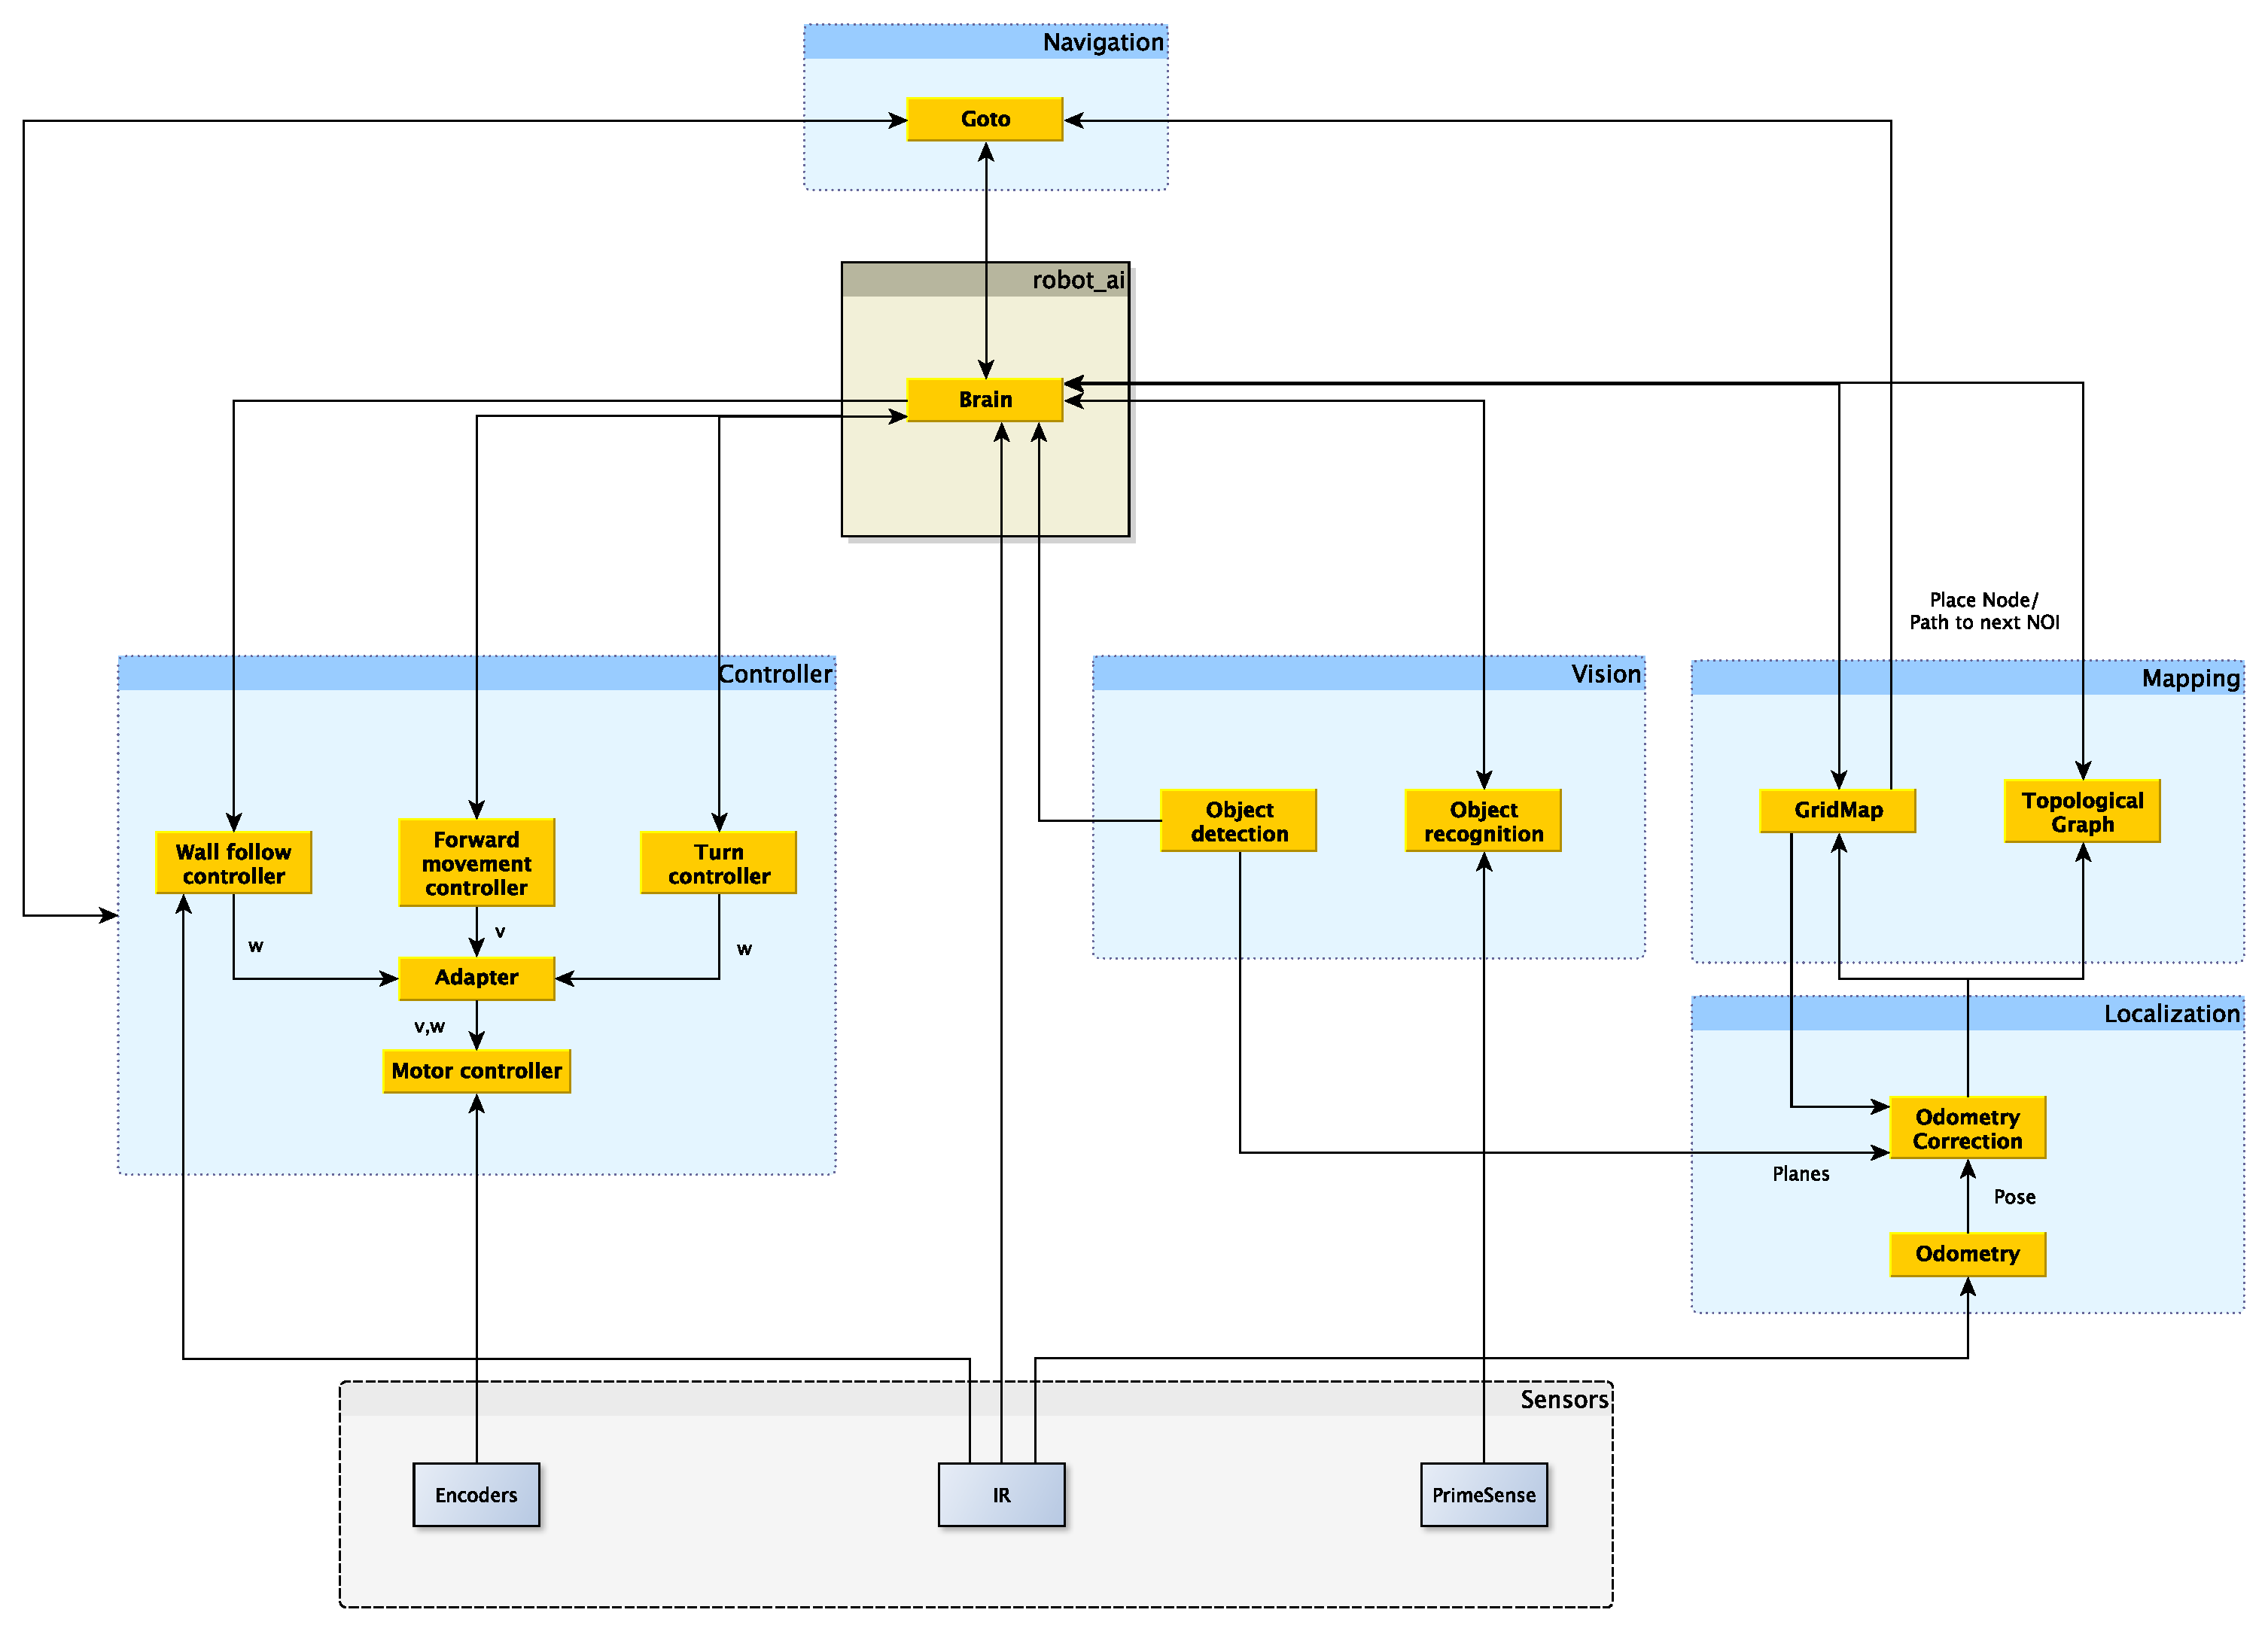
\includegraphics[width=\linewidth]{figures/architecture_full.pdf}
    }
    \caption{Main architecture of the system}
    \label{fig:1st_architecture}
\end{sidewaysfigure}

\end{appendix}

%----------------------------------------------------------------------------------------
%	BIBLIOGRAPHY
%----------------------------------------------------------------------------------------

\bibliographystyle{unsrt}

\bibliography{references}

%----------------------------------------------------------------------------------------

\end{document}